%!TEX root = ../report.tex
\chapter{System Context}
\label{ch:context}

In this chapter the context of Docker is presented.%Improve 

\subsection{System Context}
In this subsection an overview and global information about Docker purpose and history are presented. %Improve

Docker is an open-source-software designed with the purpose of making the deployment of distributed applications easier.
\begin{quote}
It automates the deployment of applications inside software containers, by providing an additional layer of abstraction and automation of operating-system-level virtualization on Linux. %\cite{•}
\end{quote}
%" Docker provides an integrated technology suite that enables development and IT operations teams to build, ship, and run distributed applications anywhere."
Docker was released as open source in March 2013. As of December 13, 2015, the project had nearly 27,000 GitHub stars (making it the 20th most-starred GitHub project), over 7,300 forks, and nearly 1,250 contributors \cite{dockerrepo}.
It's written in the Go Programming language. \\

% References
%Sources : \textit{https://www.docker.com/what-docker} \\
%\textit{https://en.wikipedia.org/wiki/Docker_28software29#History}

\begin{figure}[H]
\centering
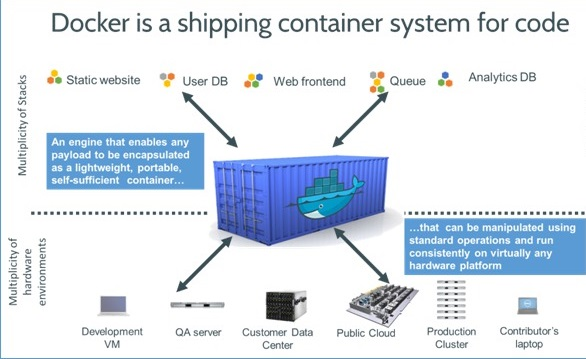
\includegraphics[scale=0.8]{images/docker_container.jpeg}
\caption{Docker}
\label{fig:analysis-mvc}
\end{figure}

\subsection{Community}
In this subsection the developpers programming docker and the community around them are presented. \\
The creator of Docker is Solomon Hykes. \\
Docker has an active community and the managers encourage developpers around the world to contribute. 
%https://docs.docker.com/opensource/project/who-written-for/
Docker started as an internal project within dotCloud, a platform-as-a-service company with four main developpers. \\
The following organizations are the main contributors to Docker: the Docker team, Red Hat, IBM, Google, Cisco Systems and Amadeus IT Group. \\

% Always quote and reference https://www.docker.com/docker-community